\section{问题三模型的建立与求解}
\label{sec:problem3}

\subsection{问题分析与建模思路}

问题三在总算力约束下联合配置参数量、训练数据量和数据质量。经典标度律描述参数量与训练 Token 数对损失的幂律作用\cite{kaplan2020scaling,hoffmann2022compute}；本问进一步把质量提升和长文本注意力纳入统一预算，考察三类资源竞争及跨预算结构转移。

问题一给出 $17$ 个领域的参考配比 $\boldsymbol p_{\mathrm{ref}}$，问题二给出广义标度律。由于现有检验只支持固定配比接口，本问不再优化十七维配比，而令

\begin{equation}
\boldsymbol p=\boldsymbol p_{\mathrm{ref}},
\qquad
D_i=p_{\mathrm{ref},i}D,\quad i=1,\ldots,17.
\label{eq:p3_fixed_mixture}
\end{equation}

即先优化总 Token 数 $D$，再分解到各领域。决策量为 $N,D,Q_A$，预算 $C$、上下文 $L_{\mathrm{ctx}}$ 与质量成本 $g$ 为外生情景。利用损失关于 $D$ 严格递减的性质，可解析消去 $D$，再通过多起点精化、预算追踪和三维复核求解，并由 KKT 条件与配置弹性解释结构转移。

总体路线见图~\ref{fig:p3_solver_flow}：从前两问冻结接口出发，依次完成可行性判断、二维求解、三维复核、成本回代及 KKT 与抽样检验，再将验收通过的情景发布给问题四；具体计算顺序见算法~\ref{alg:p3_solver}。

\begin{figure}[H]
\centering
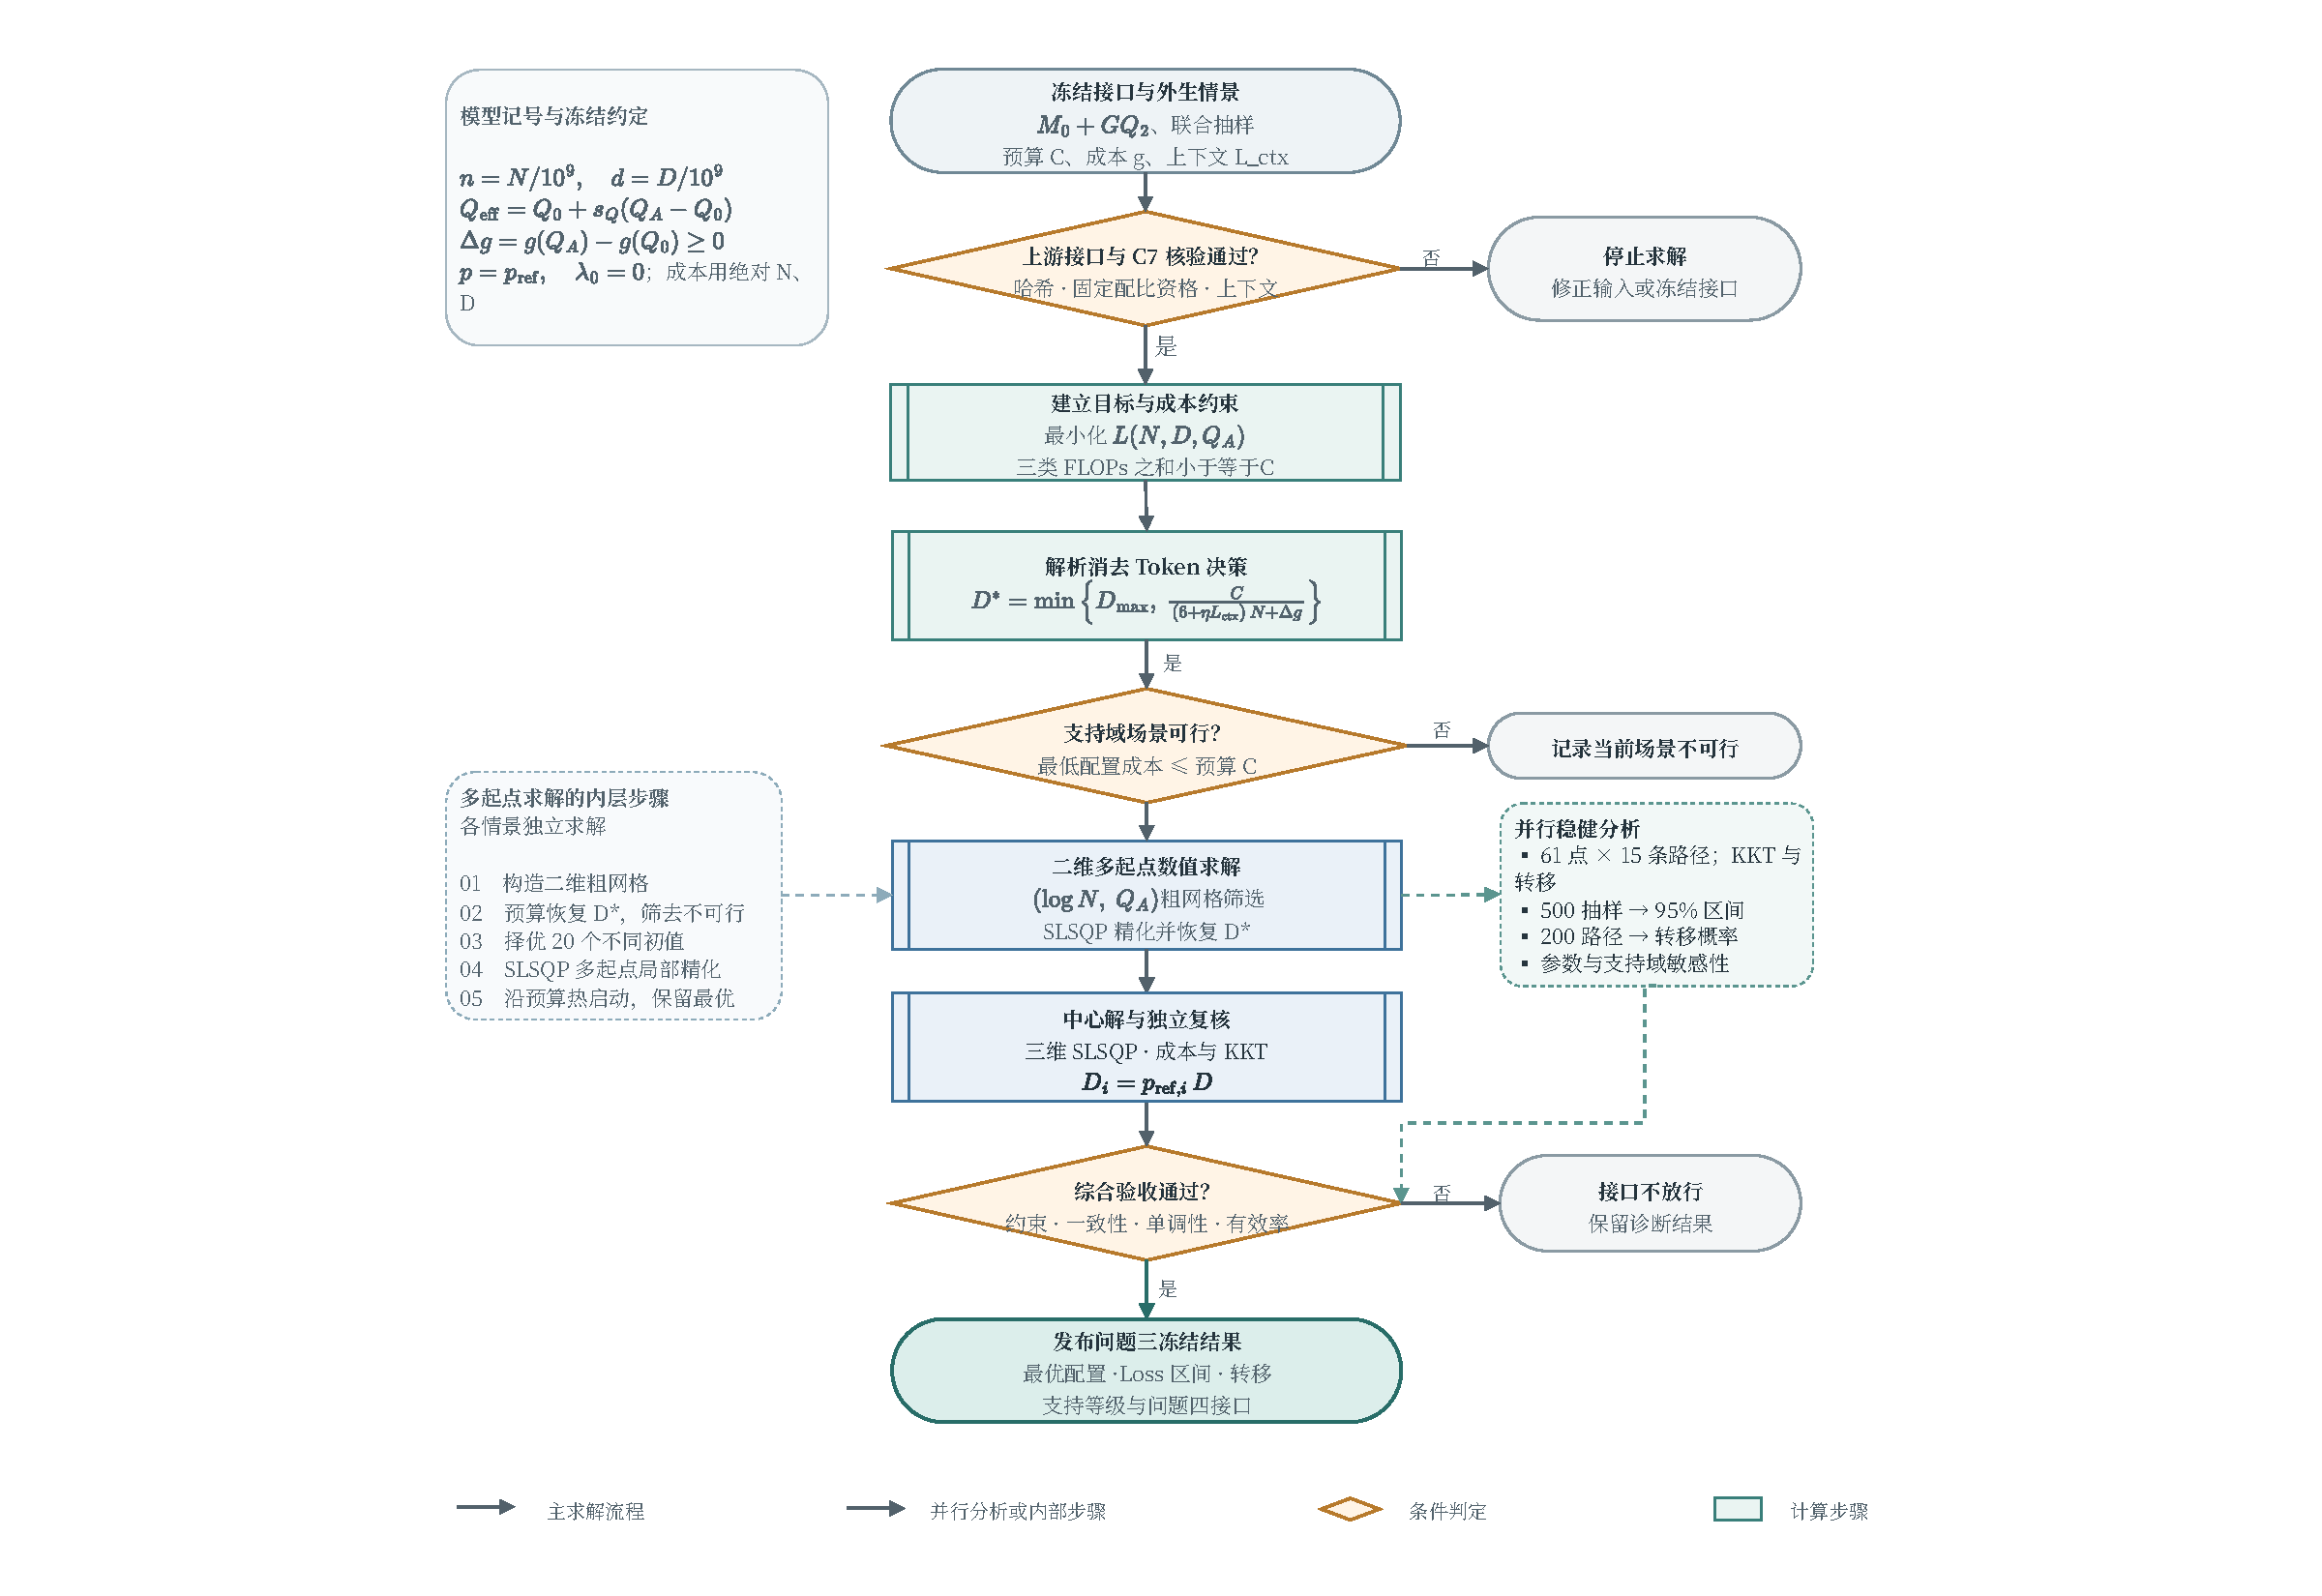
\includegraphics[width=0.78\linewidth,trim=0 90bp 0 0,clip]{images/no3/P3_F00R_问题三资源配置求解流程图.pdf}
\caption{问题三资源配置优化的求解、复核与验收流程}
\label{fig:p3_solver_flow}
\end{figure}

\subsection{资源配置模型的建立}

\subsubsection{冻结输入与决策边界}

本问沿用问题二的参数--数据可分标度律与加性质量惩罚模型，不重复拟合附件 A、B；其基础训练轨迹来自 Pythia 模型族\cite{biderman2023pythia}。将冻结预测 $\widehat L_{\mathrm{main}}$ 简记为

\begin{equation}
L(N,D,Q_A)
=E+A\left(\frac{N}{10^9}\right)^{-\alpha}
+B\left(\frac{D}{10^9}\right)^{-\beta}
+c_Q(1-Q_{\mathrm{eff}})^{\nu_Q},
\label{eq:p3_generalized_scaling}
\end{equation}

其中 $Q_{\mathrm{eff}}$ 为进入损失函数的有效质量。两问的质量变量来自不同实验体系，故以公共参考质量 $Q_0$ 为锚点，作线性对齐并限制其不超过有效上界：

\begin{equation}
\begin{aligned}
Q_{\mathrm{eff}}&=Q_0+s_Q(Q_A-Q_0),
\qquad Q_0=0.5389559588,\\
Q_{\mathrm{sat}}&=\min\left\{1,
Q_0+\frac{1-\varepsilon-Q_0}{s_Q}\right\},
\qquad \varepsilon=10^{-6}.
\end{aligned}
\label{eq:p3_quality_mapping}
\end{equation}

主情景取 $s_Q=1$，并以 $0.5$ 和 $1.5$ 检验跨体系映射敏感性。式~\eqref{eq:p3_generalized_scaling} 的参数沿用问题二中心估计；在合法区间内，增大 $N$、$D$ 或 $Q_A$ 均不会使预测损失上升。表~\ref{tab:p3_interface} 汇总优化接口，避免冻结量、决策量与情景量混用。

\begin{table}[!htbp]
\centering
\small
\setlength{\tabcolsep}{5pt}
\caption{问题三的冻结输入、决策变量与情景变量}
\label{tab:p3_interface}
\begin{tabular}{p{0.18\linewidth}p{0.30\linewidth}p{0.42\linewidth}}
\toprule
类型 & 变量 & 来源或作用 \\
\midrule
冻结输入 & $\boldsymbol p_{\mathrm{ref}},Q_0,E,A,B,\alpha,\beta,c_Q,\nu_Q$ & 由问题一和问题二传入，优化中不重估 \\
决策变量 & $N,D,Q_A$ & 在给定算力预算下最小化冻结 Loss \\
情景变量 & $C,L_{\mathrm{ctx}},g,s_Q$ & 描述预算、上下文、质量成本与映射假设 \\
派生输出 & $D_i=p_{\mathrm{ref},i}D^*$ & 将最优总 Token 数分解到 $17$ 个领域 \\
\bottomrule
\end{tabular}
\end{table}

\subsubsection{三类算力成本与优化约束}

基础训练、质量提升和长文本注意力三类成本分别定义为

\begin{equation}
\begin{aligned}
C_{\mathrm{train}}&=6ND,\\
C_Q&=D\,[g(Q_A)-g(Q_0)]_+,\\
C_{\mathrm{attn}}&=\eta NDL_{\mathrm{ctx}},
\qquad \eta=2\times10^{-4},
\end{aligned}
\label{eq:p3_three_costs}
\end{equation}

其中 $[x]_+=\max(x,0)$，$6ND$ 为常用训练算力近似\cite{kaplan2020scaling,hoffmann2022compute}。自注意力对序列长度具有二次复杂度\cite{vaswani2017attention}；固定总 Token 数后，每个 Token 的附加开销近似正比于上下文长度，故用 $\eta NDL_{\mathrm{ctx}}$ 表示。系数 $\eta$ 为题设情景参数。三种质量成本取

\begin{equation}
\begin{aligned}
g_{\exp}(Q)&=10^7e^{6Q},\\
g_{\mathrm{pow}}(Q)&=5\times10^9Q^4,\\
g_{\log}(Q)&=2\times10^9\ln(1+10Q).
\end{aligned}
\label{eq:p3_quality_costs}
\end{equation}

三种形式表示不同的质量处理成本情景，并非重新拟合的候选模型，故只作并列条件比较。综合上述定义，优化模型为

\begin{equation}
\begin{aligned}
\min_{N,D,Q_A}\quad
&L(N,D,Q_A),\\
\text{s.t.}\quad
&6ND+D[g(Q_A)-g(Q_0)]_+
+\eta NDL_{\mathrm{ctx}}\le C,\\
&N_{\min}\le N\le N_{\max},\\
&D_{\min}\le D\le D_{\max},\\
&Q_0\le Q_A\le Q_{\mathrm{sat}}.
\end{aligned}
\label{eq:p3_optimization}
\end{equation}

成本式中的 $N,D$ 使用绝对数量；式~\eqref{eq:p3_generalized_scaling} 中除以 $10^9$ 仅用于无量纲化，不能把十亿单位直接代入成本式。

\subsubsection{上下文情景与支持域}

附件 C7 的 $45$ 条记录形成 $2048$、$4096$、$8192$、$32768$ 和 $131072$ 五档上下文。鉴于部分架构字段不一致，本问只使用独立核验后的上下文窗口，并将五档视为等权外生情景。为区分观测支持内结论与外推结果，设置

\begin{equation}
\begin{array}{lll}
\text{严格共同支持域：}&N\in[0.070542,11.965825]\ \mathrm{B},
&D\in[10,299.893]\ \mathrm{B},\\
\text{条件扩展域：}&N\in[0.070542,10000]\ \mathrm{B},
&D\in[0.1,36000]\ \mathrm{B}.
\end{array}
\label{eq:p3_support_domains}
\end{equation}

严格域用于检验参数项和质量项均有数据覆盖的结果，扩展域用于回答三档预算。每个解标记为共同观测支持、单分量外推、桥接缺口外推或边界支持外推；严格域不可行时如实报告，超出扩展域的方案判为无效。

\subsection{模型求解}

\subsubsection{解析降维与多起点优化}

将总成本写成

\begin{equation}
C_{\mathrm{tot}}
=D\left[(6+\eta L_{\mathrm{ctx}})N
+\Delta g(Q_A)\right],
\qquad
\Delta g(Q_A)=[g(Q_A)-g(Q_0)]_+.
\label{eq:p3_cost_rearranged}
\end{equation}

由式~\eqref{eq:p3_generalized_scaling} 可知，固定 $(N,Q_A)$ 时有 $\partial L/\partial D<0$，因此应把剩余预算全部用于增加训练 Token 数。预算允许的最大数据量为

\begin{equation}
D^{\max}(N,Q_A)
=\frac{C}{(6+\eta L_{\mathrm{ctx}})N+\Delta g(Q_A)},
\label{eq:p3_dmax}
\end{equation}

考虑搜索上界后取

\begin{equation}
D^*(N,Q_A)
=\min\{D_{\max},D^{\max}(N,Q_A)\},
\qquad D^*(N,Q_A)\ge D_{\min}.
\label{eq:p3_dstar}
\end{equation}

三维约束优化由此降为 $(\log N,Q_A)$ 上的二维有界优化。每个成本函数、上下文、预算、质量映射和支持域组合均先进行粗网格搜索，再从目标值最小的二十个不同网格点出发作局部精化；沿预算递增方向，以上一预算的最优解作为连续追踪初值。三档预算、三种成本和五档上下文构成的 $45$ 个中心情景，另用完整三维非线性规划独立求解，并以加密网格检查局部最优风险。

图~\ref{fig:p3_low_budget_landscape} 以 $4096$ 上下文和 $10^{19}$ FLOPs 为例展示降维后的目标景观。三个谷底均体现参数量与质量的替代关系，但不同质量成本改变了谷底沿 $Q_A$ 方向的位置：指数成本形成内点解，幂函数成本停留在质量基线，对数成本则到达质量上界。这也说明多起点搜索和边界识别不可省略。

\begin{figure}[!htbp]
\centering
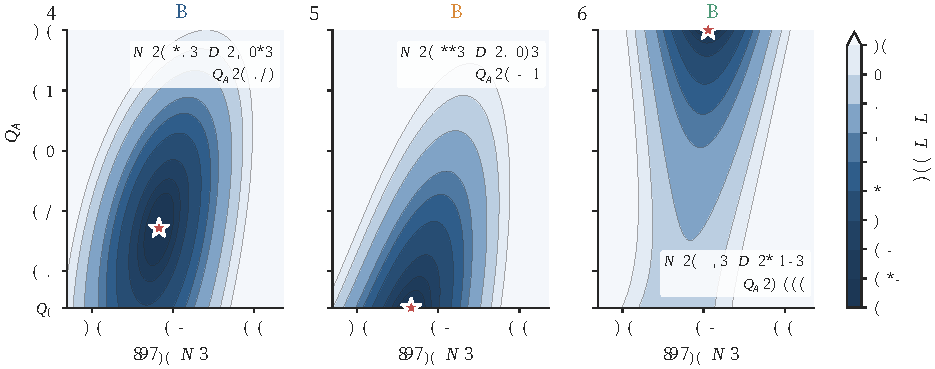
\includegraphics[width=0.94\linewidth]{images/no3/P3_F03_三类质量成本下的低预算优化景观.pdf}
\caption{$4096$ 上下文、$10^{19}$ FLOPs 下三类质量成本的解析降维景观}
\label{fig:p3_low_budget_landscape}
\end{figure}

在实现层面，算法~\ref{alg:p3_solver} 给出二维求解、三维复核、预算连续追踪和结构转移筛选的可复现顺序。

\begin{algorithm}[!htbp]
\caption{算力约束下资源配置与结构转移识别}
\label{alg:p3_solver}
\begin{algorithmic}[1]
\Require 冻结参数 $\boldsymbol\theta$、参考配比 $\boldsymbol p_{\mathrm{ref}}$、预算 $\mathcal C$、上下文 $\mathcal L$、成本集合 $\mathcal G$、支持域 $\mathcal S$
\Ensure 中心最优解、领域 Token 配置、活跃约束与稳定转移点
\ForAll{$g\in\mathcal G$，$L_{\mathrm{ctx}}\in\mathcal L$，$\mathcal S$}
    \ForAll{按升序排列的 $C\in\mathcal C$}
        \State 由式~\eqref{eq:p3_dstar} 计算粗网格，并删除不可行点
        \State 取最优的 $20$ 个网格点和上一预算解作为初值
        \State 对各初值执行二维有界局部精化，取 Loss 最小的可行解 $\boldsymbol x^*(C)$
        \If{$C\in\{10^{19},10^{22},10^{24}\}$}
            \State 使用完整三维非线性规划与加密网格独立复核 $\boldsymbol x^*(C)$
        \EndIf
        \State 记录成本份额、支持状态及 $D_i=p_{\mathrm{ref},i}D^*$
    \EndFor
\State 比较相邻预算的活跃集合，并用配置弹性与 BIC 筛选次要断点
\EndFor
\State 以 $500$ 次锚点 bootstrap 和 $200$ 条联合抽样路径传播不确定性
\State 输出出现概率不低于 $70\%$ 的结构转移
\end{algorithmic}
\end{algorithm}

当 $Q_A=Q_0$ 且变量边界均未激活时，令 $n=N/10^9$、$d=D/10^9$、$\overline C=C/[(6+\eta L_{\mathrm{ctx}})10^{18}]$，不含质量投资的部分具有闭式基准

\begin{equation}
n^*
=\left(\frac{\alpha A}{\beta B}\right)^{1/(\alpha+\beta)}
\overline C^{\beta/(\alpha+\beta)},
\qquad
d^*=\frac{\overline C}{n^*}.
\label{eq:p3_classic_closed_form}
\end{equation}

该结果仅用于初始化和公式回归，不替代正式优化结果。

\subsubsection{KKT边际解释}

在满足约束资格条件、预算约束活跃且三类决策均位于内点时，KKT 必要条件要求三种资源的单位算力边际收益相等\cite{nocedal2006numerical}：

\begin{equation}
\frac{-L_N}{C_N}
=\frac{-L_D}{C_D}
=\frac{-L_Q}{C'_Q},
\label{eq:p3_kkt_ratio}
\end{equation}

其中

\begin{equation}
\begin{aligned}
C_N&=(6+\eta L_{\mathrm{ctx}})D,\\
C_D&=(6+\eta L_{\mathrm{ctx}})N+\Delta g(Q_A),\\
C'_Q&=Dg'(Q_A).
\end{aligned}
\label{eq:p3_marginal_costs}
\end{equation}

式~\eqref{eq:p3_kkt_ratio} 给出了资源配置的直接解释：若质量下界乘子为正，则当前预算下新增算力投入质量不如投入参数或 Token；当该乘子降为零并且 $Q_A$ 离开 $Q_0$ 时，质量投资才被启用；当 $Q_A$ 达到 $Q_{\mathrm{sat}}$ 后，新增预算重新主要流向参数和数据扩张。

\subsubsection{结构性转移的数学定义}

固定质量成本、上下文、质量尺度和支持域，定义预算 $C$ 下最优解的活跃集合

\begin{equation}
\mathcal A(C)=
\{Q_A=Q_0,\ Q_A=Q_{\mathrm{sat}},\
N=N_{\min/\max},\ D=D_{\min/\max},\
C_{\mathrm{tot}}=C\}.
\label{eq:p3_active_set}
\end{equation}

若临界预算两侧满足 $\mathcal A(C^-)\neq\mathcal A(C^+)$，则记为主要转移；对活跃集合不变的区段，再计算配置弹性

\begin{equation}
\theta_x(C)=\frac{\mathrm d\log x^*}{\mathrm d\log C},
\qquad x\in\{N,D,Q_A-Q_0\}.
\label{eq:p3_configuration_elasticity}
\end{equation}

分段线性拟合相对单直线的 BIC 改善不低于 $10$ 且断点两侧斜率差不低于 $0.15$ 时，记为次要候选\cite{schwarz1978estimating}。转移点由 $61$ 个对数预算点夹逼，主要转移再二分至 $\log_{10}C$ 区间宽度不超过 $0.01$；同类事件在至少 $70\%$ 的抽样路径中出现时，才称为稳定转移。

\subsection{结果分析与模型验证}

\subsubsection{上下文临界长度}

由式~\eqref{eq:p3_three_costs} 可知，注意力成本和基础训练成本之比为

\begin{equation}
\frac{C_{\mathrm{attn}}}{C_{\mathrm{train}}}
=\frac{\eta L_{\mathrm{ctx}}}{6}.
\label{eq:p3_attention_ratio}
\end{equation}

令该比值等于 $1$，得到两类成本相等的临界上下文长度

\begin{equation}
L_{\mathrm{ctx}}^{\mathrm{crit}}
=\frac{6}{\eta}=30000.
\label{eq:p3_context_critical}
\end{equation}

五档上下文对应的上述比值依次为 $0.0683$、$0.1365$、$0.2731$、$1.0923$ 和 $4.3691$，故后两档已经越过临界点。图~\ref{fig:p3_context_penalty} 进一步以 $2048$ Token 为基准，比较上下文增长带来的最优 Loss 增量。

\begin{figure}[!htbp]
\centering
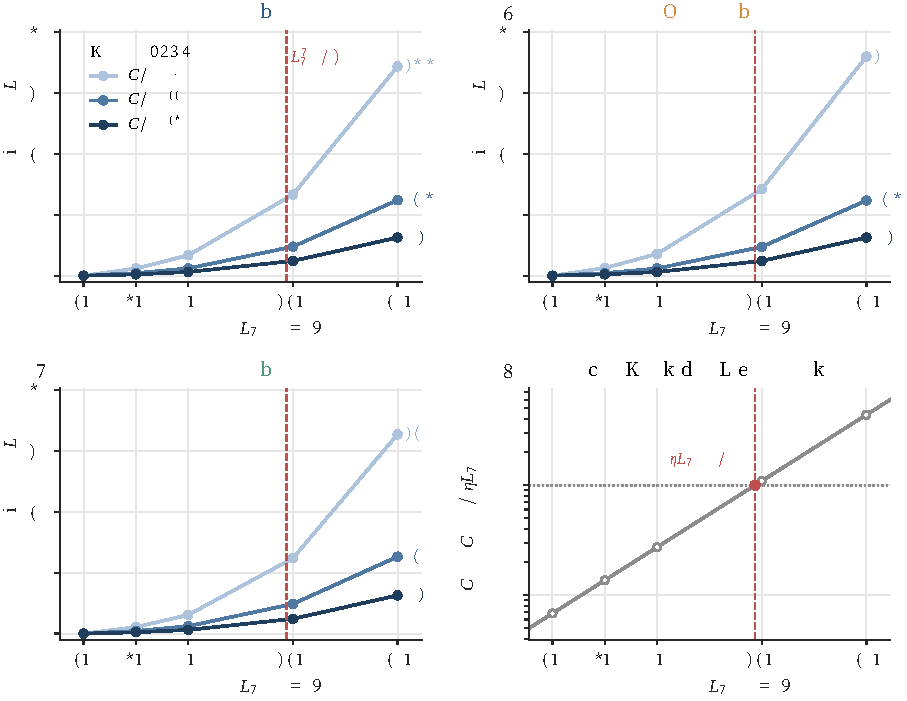
\includegraphics[width=0.94\linewidth]{images/no3/P3_F02_上下文成本临界与最优损失惩罚.pdf}
\caption{上下文长度引起的最优 Loss 增量与 $30000$ Token 临界线}
\label{fig:p3_context_penalty}
\end{figure}

跨过 $30000$ Token 后，三类成本情景的惩罚均明显扩大；在 $131072$ Token 下，$10^{19}$ FLOPs 的 $100\Delta L$ 达 $32.7$--$36.0$，而 $10^{24}$ FLOPs 约为 $6.3$。长上下文会挤压低预算下本已有限的参数和数据投入，高预算则能通过扩大规模部分吸收影响。需注意，式~\eqref{eq:p3_attention_ratio} 与预算及最优解无关，因此 $30000$ 描述上下文成本临界，而非随预算增加产生的结构转移。

最优 Loss 的变化来自最优配置的内生调整。图~\ref{fig:p3_context_response} 将 $N^*$ 和 $D^*$ 分别对 $2048$ Token 情景归一化，并同时给出质量决策 $Q_A^*$。

\begin{figure}[!htbp]
\centering
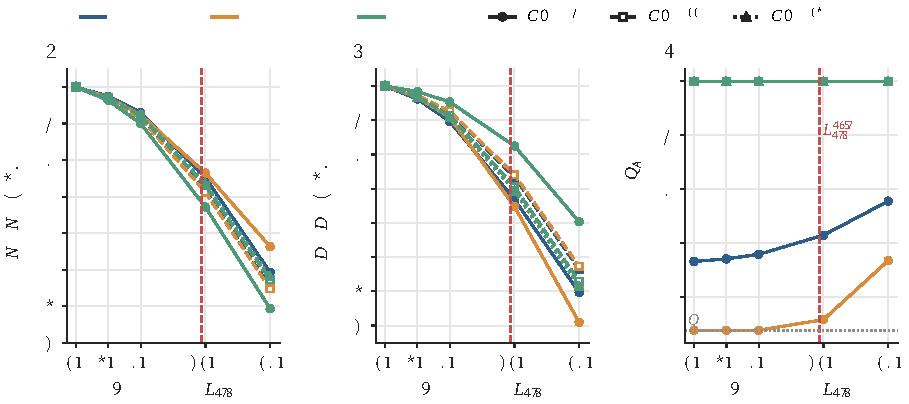
\includegraphics[width=0.94\linewidth]{images/no3/P3_F04_上下文长度对最优配置的影响.pdf}
\caption{上下文长度对三类质量成本最优配置的影响}
\label{fig:p3_context_response}
\end{figure}

参数量和 Token 量均随上下文增长而下降，且数据量通常压缩更快。以低预算指数成本为例，$131072$ Token 时 $N^*$、$D^*$ 分别降至基准的 $49.3\%$、$39.7\%$，而 $Q_A^*$ 由 $0.666$ 升至 $0.778$。未饱和时，提高质量可部分对冲规模收缩；质量饱和后，长上下文成本只能由 $N^*$ 与 $D^*$ 共同吸收。

\subsubsection{三档预算下的最优资源配置}

以 $L_{\mathrm{ctx}}=4096$、$s_Q=1$ 和条件扩展域为主展示情景，三档预算下的中心最优配置见表~\ref{tab:p3_anchor_allocations}。表中 $N$ 和 $D$ 均以十亿为单位；为突出问题三的资源配置结论，仅保留最优决策、预测 Loss 和支持状态，三类成本份额在正文中解释。

\begin{table}[!htbp]
\centering
\caption{4096上下文下三档预算的中心最优配置}
\label{tab:p3_anchor_allocations}
\footnotesize
\setlength{\tabcolsep}{3.5pt}
\begin{tabular}{llrrrrl}
\toprule
质量成本 & 预算/FLOPs & $N^*$ & $D^*$ & $Q_A^*$ & $L^*$ & 支持状态 \\
\midrule
指数 & $10^{19}$ & $0.259187$ & $4.82101$ & $0.671056$ & $3.16898$ & 单分量外推 \\
指数 & $10^{22}$ & $5.44886$ & $244.275$ & $0.999999$ & $2.15491$ & 共同观测支持 \\
指数 & $10^{24}$ & $39.5804$ & $3653.81$ & $0.999999$ & $1.91601$ & 桥接缺口外推 \\
\midrule
幂函数 & $10^{19}$ & $0.215205$ & $6.81420$ & $0.538956$ & $3.17962$ & 单分量外推 \\
幂函数 & $10^{22}$ & $5.55840$ & $235.394$ & $0.999999$ & $2.15634$ & 共同观测支持 \\
幂函数 & $10^{24}$ & $39.7119$ & $3631.33$ & $0.999999$ & $1.91611$ & 桥接缺口外推 \\
\midrule
对数 & $10^{19}$ & $0.337313$ & $2.95276$ & $0.999999$ & $3.11805$ & 单分量外推 \\
对数 & $10^{22}$ & $5.04774$ & $281.627$ & $0.999999$ & $2.14976$ & 共同观测支持 \\
对数 & $10^{24}$ & $39.1302$ & $3732.41$ & $0.999999$ & $1.91566$ & 桥接缺口外推 \\
\bottomrule
\end{tabular}
\end{table}

低预算下三类路径差异最大，与图~\ref{fig:p3_low_budget_landscape} 的谷底位置一致：指数成本选择内点质量 $Q_A=0.671056$，幂函数成本停留在 $Q_0$，对数成本达到质量上界并以 $32.08\%$ 的预算提质。其 Loss 最低只表示该题设成本下的条件结果，不能反推真实质量处理必然服从对数成本。三种低预算解均属单分量外推，主要用于比较机制。

预算提高到 $10^{22}$ FLOPs 后，三类成本均达到质量上界且处于共同观测支持域；到 $10^{24}$ FLOPs，最优参数量约为 $39.1$--$39.7$ B、数据量约为 $3.63$--$3.73$ 万亿 Token，三类 Loss 差异小于 $5\times10^{-4}$。这表明质量饱和后，新增预算重新流向参数和数据扩张，成本函数形状的影响迅速减弱。

每个方案再按式~\eqref{eq:p3_fixed_mixture} 分解为十七个领域的 Token 数，满足 $D_i\ge0$ 和 $\sum_iD_i=D$，从而把最优总数据量转化为可执行的领域预算。

\subsubsection{连续预算路径与成本份额}

在 $4096$ 上下文的连续预算路径上，$N^*$ 和 $D^*$ 总体近似幂律增长，而质量路径呈阶段差异：对数成本从起点即饱和，指数成本从中等质量继续上升，幂函数成本则先保持基线再启动提质。

\begin{figure}[!htbp]
\centering
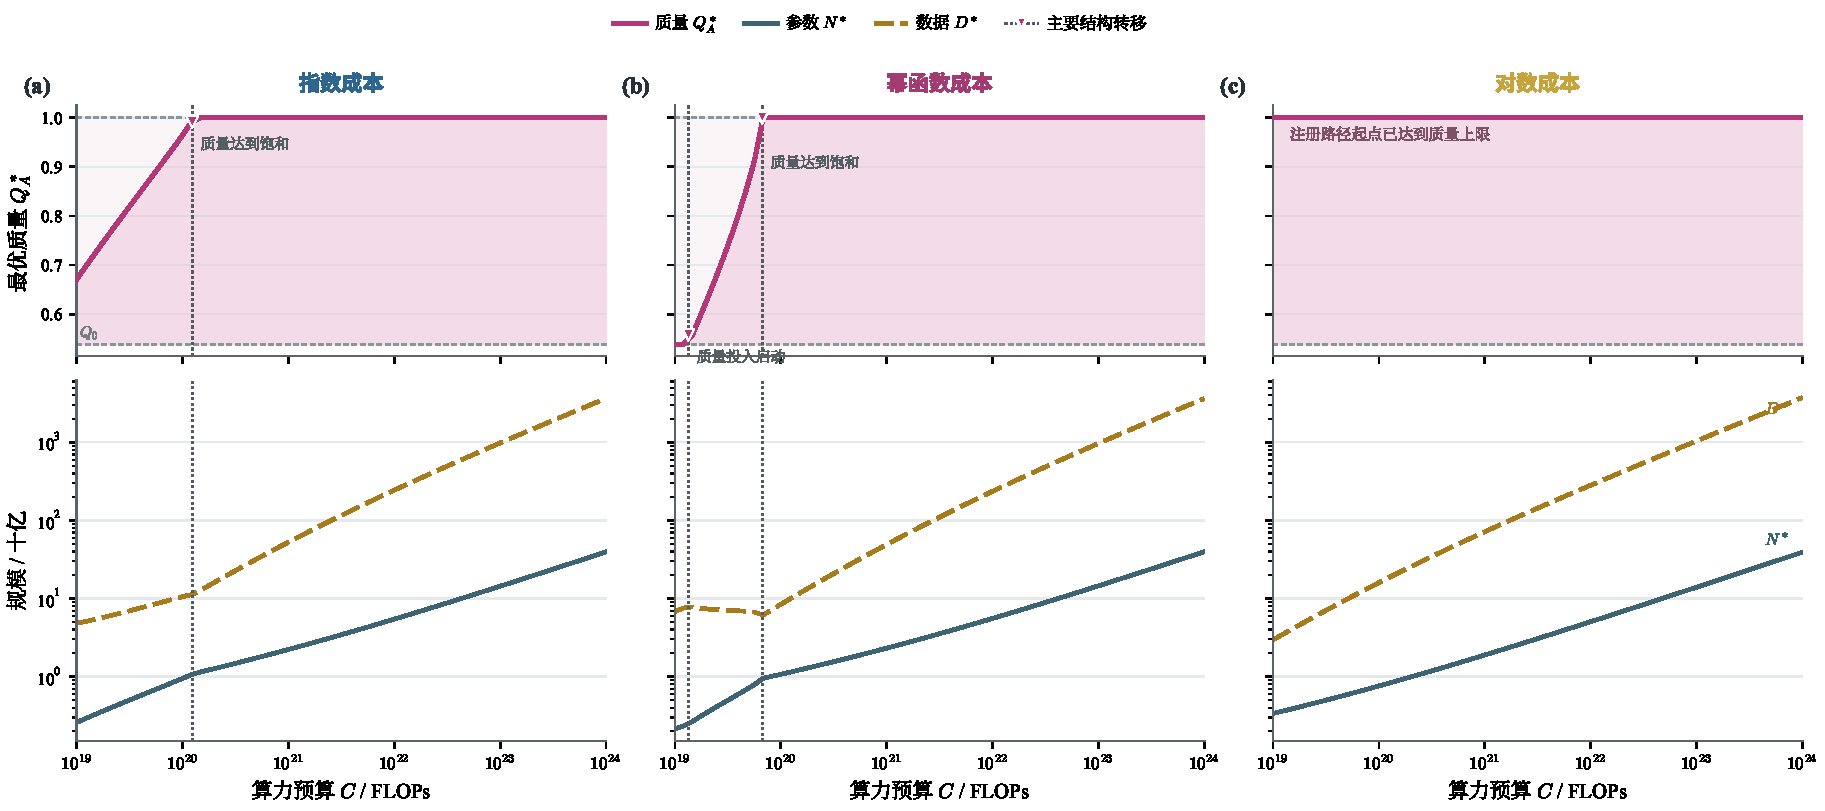
\includegraphics[width=0.94\linewidth]{images/no3/P3_F07_最优配置路径与结构转移.pdf}
\caption{$4096$ 上下文下的连续最优配置路径与结构转移}
\label{fig:p3_configuration_paths}
\end{figure}

图~\ref{fig:p3_configuration_paths} 将质量状态与参数--Token 扩张对齐。幂函数路径在 $1.342\times10^{19}$ FLOPs 离开 $Q_0$、在 $6.691\times10^{19}$ FLOPs 饱和；指数路径在 $1.234\times10^{20}$ FLOPs 饱和。质量曲线变平后 $N^*$ 与 $D^*$ 仍增长，说明新增预算已转回规模扩张。

固定上下文时，注意力与基础训练成本的相对比例不变，因此份额变化主要来自质量成本与规模成本的竞争。指数和幂函数情景的质量份额先升后降，对数情景则从高位单调下降；高预算区间均由基础训练成本主导。

\begin{figure}[!htbp]
\centering
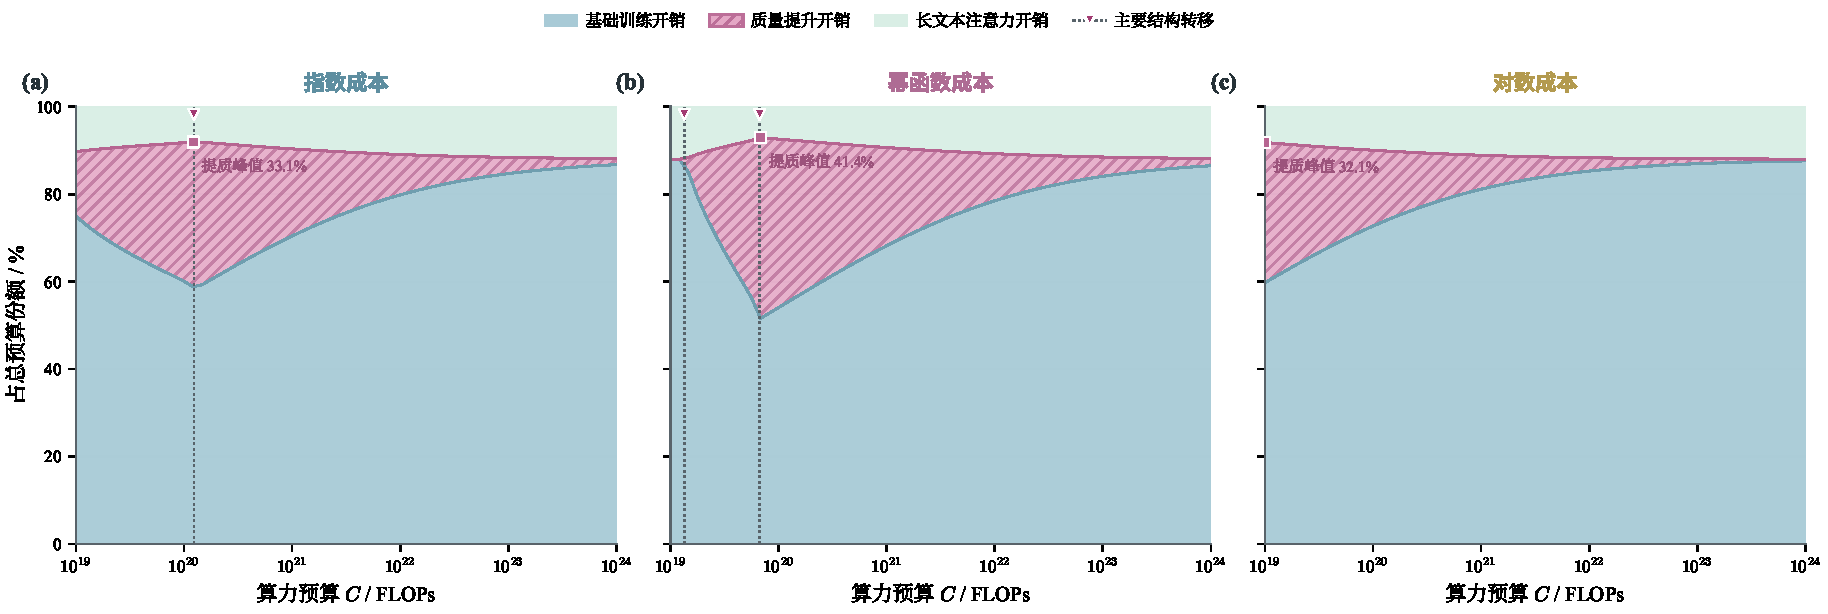
\includegraphics[width=0.94\linewidth]{images/no3/P3_F01_预算约束下的边际资源竞争机制.pdf}
\caption{$4096$ 上下文下连续预算路径的算力份额分解}
\label{fig:p3_budget_shares}
\end{figure}

图~\ref{fig:p3_budget_shares} 中三类质量份额峰值分别约为 $33.1\%$、$41.4\%$ 和 $32.1\%$。质量带的扩张与收缩直接对应式~\eqref{eq:p3_kkt_ratio} 的边际竞争；达到上限后，其份额被持续增长的规模成本稀释。

\subsubsection{稳定结构性转移}

$4096$ 上下文下通过稳定性门槛的转移见表~\ref{tab:p3_transitions}。指数成本依次出现质量弹性断点、质量饱和和数据量弹性断点；幂函数成本则完整经历“保持基线--启动提质--质量饱和--规模扩张”，具体临界预算由表中给出。

\begin{table}[!htbp]
\centering
\caption{4096上下文下的稳定结构性转移}
\label{tab:p3_transitions}
\small
\setlength{\tabcolsep}{5pt}
\begin{tabular}{lllrr}
\toprule
质量成本 & 层级 & 转移事件 & 临界预算/FLOPs & 出现概率 \\
\midrule
指数 & 次要 & 质量增量弹性断点 & $9.085\times10^{19}$ & $1.000$ \\
指数 & 主要 & 质量达到饱和 & $1.234\times10^{20}$ & $1.000$ \\
指数 & 次要 & 数据量弹性断点 & $2.371\times10^{20}$ & $1.000$ \\
\midrule
幂函数 & 主要 & 质量投资启动 & $1.342\times10^{19}$ & $1.000$ \\
幂函数 & 次要 & 质量增量弹性断点 & $4.217\times10^{19}$ & $1.000$ \\
幂函数 & 主要 & 质量达到饱和 & $6.691\times10^{19}$ & $1.000$ \\
幂函数 & 次要 & 参数量弹性断点 & $1.101\times10^{20}$ & $1.000$ \\
幂函数 & 次要 & 数据量弹性断点 & $1.101\times10^{20}$ & $1.000$ \\
\bottomrule
\end{tabular}
\end{table}

中心参数下的单一临界值不足以衡量事件定位的可靠性。图~\ref{fig:p3_transition_bootstrap} 因此同时给出两个关键转移事件在 $200$ 条联合参数路径上的二维分布及边缘分布。

\begin{figure}[!htbp]
\centering
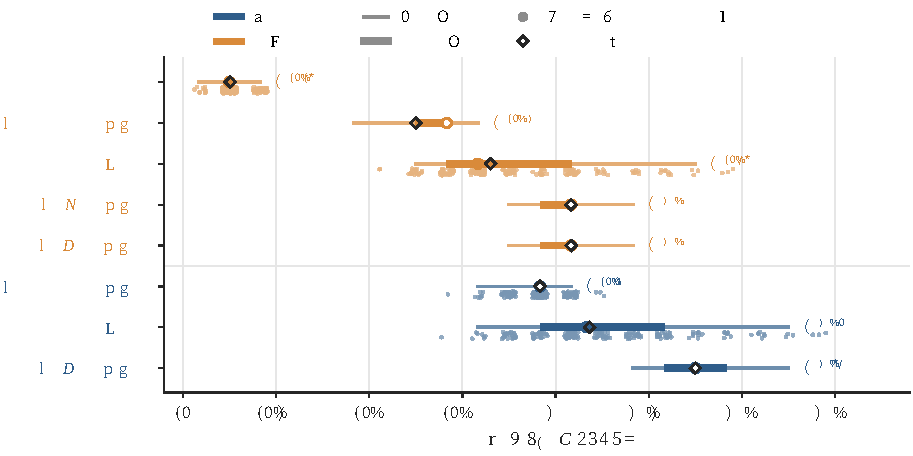
\includegraphics[width=0.92\linewidth]{images/no3/P3_F05_稳定结构转移的区间估计.pdf}
\caption{$4096$ 上下文下关键结构转移预算的联合 bootstrap 分布}
\label{fig:p3_transition_bootstrap}
\end{figure}

指数成本下，质量弹性断点与饱和位置呈较强正相关（$\rho=0.81$）；幂函数成本下启动与饱和位置的相关系数仅为 $-0.08$。中心结果均位于 bootstrap 主体区域，事件出现概率均为 $1$。主要、次要转移的 $\log_{10}C$ 定位区间宽度分别为 $0.00521$、$0.08333$。对数成本在路径起点已达质量上界，故当前预算范围内没有新的质量状态转移。

因此，资源配置可概括为三个阶段：低预算下保持质量基线，跨过阈值后质量与规模竞争，质量饱和后新增算力重新集中到参数和数据扩张。阶段边界随成本函数和上下文变化，但该机制在可行情景中一致。

\subsection{敏感性、适用边界与本问输出}

\subsubsection{参数不确定性传播}

每个中心情景以 $500$ 组联合参数 bootstrap 样本传播问题二参数和参考质量的不确定性\cite{efron1979bootstrap}。表~\ref{tab:p3_bootstrap_loss} 表明，低预算下质量参数影响较明显，幂函数成本区间最宽；质量饱和后各区间均显著收窄。

\begin{table}[!htbp]
\centering
\caption{4096上下文下最优Loss的bootstrap区间}
\label{tab:p3_bootstrap_loss}
\small
\setlength{\tabcolsep}{6pt}
\begin{tabular}{llrrr}
\toprule
质量成本 & 预算/FLOPs & 中位数 & $2.5\%$分位数 & $97.5\%$分位数 \\
\midrule
指数 & $10^{19}$ & $3.16903$ & $3.15657$ & $3.18222$ \\
指数 & $10^{22}$ & $2.15491$ & $2.15488$ & $2.15493$ \\
指数 & $10^{24}$ & $1.91601$ & $1.91595$ & $1.91607$ \\
\midrule
幂函数 & $10^{19}$ & $3.18002$ & $3.16432$ & $3.19592$ \\
幂函数 & $10^{22}$ & $2.15634$ & $2.15631$ & $2.15636$ \\
幂函数 & $10^{24}$ & $1.91611$ & $1.91605$ & $1.91617$ \\
\midrule
对数 & $10^{19}$ & $3.11805$ & $3.11728$ & $3.11871$ \\
对数 & $10^{22}$ & $2.14975$ & $2.14972$ & $2.14978$ \\
对数 & $10^{24}$ & $1.91567$ & $1.91560$ & $1.91572$ \\
\bottomrule
\end{tabular}
\end{table}

连续预算路径另分层选取 $200$ 组联合样本估计转移概率，以保留 $E,A,B,\alpha,\beta,c_Q,\nu_Q$ 与 $Q_0$ 之间的相关结构。

\subsubsection{敏感性与证据边界}

敏感性分析包含 $234$ 个场景，覆盖质量映射斜率、质量成本与注意力系数的 $\pm20\%$ 扰动、经验质量上界及严格共同支持域。质量映射主要影响低预算下是否启动提质；质量饱和后，Loss 对该斜率的敏感性明显降低。

\begin{figure}[!htbp]
\centering
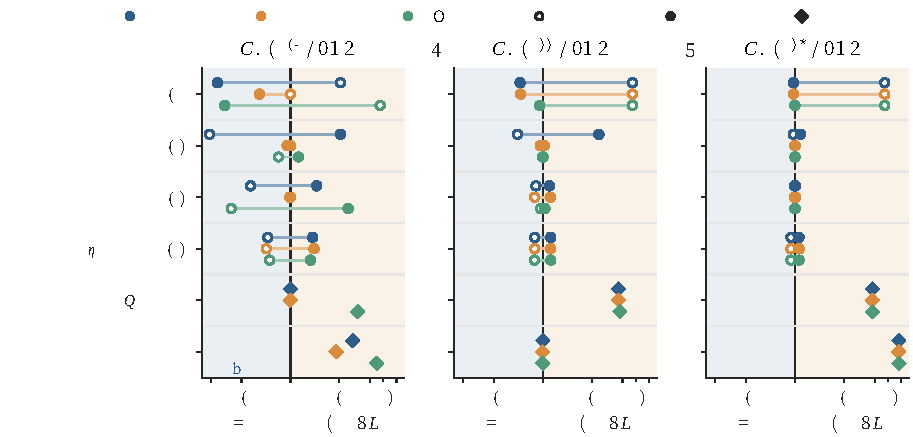
\includegraphics[width=0.92\linewidth]{images/no3/P3_F06_关键假设的敏感性分析.pdf}
\caption{$4096$ 上下文下关键假设对最优 Loss 的敏感性}
\label{fig:p3_sensitivity}
\end{figure}

图~\ref{fig:p3_sensitivity} 中，$10^{19}$ FLOPs 下点位最分散；到 $10^{22}$ 和 $10^{24}$ FLOPs，多数双侧扰动收缩到零附近。严格支持域检查在高预算下仍使 Loss 明显上升，这是扩展域最优规模被观测边界截断所致，而非局部参数不稳定。

$45$ 个中心情景中有 $30$ 个带外推标记：$10^{19}$ FLOPs 主要为单分量外推，$10^{22}$ FLOPs 主展示结果位于共同观测支持域，$10^{24}$ FLOPs 则跨越桥接缺口。因此，高预算结果属于冻结标度律边界内的条件推断，而非新增实测证据。

\subsubsection{数值验收}

本文逐项回代成本、边界、单位、预算、二维--三维一致性、加密网格与领域 Token 守恒。Loss 重建误差和同种子重复相对差均为 $0$；约束违反量、二维--三维 Loss 相对差、加密网格相对差和 Token 求和误差分别为 $4.096\times10^{-16}$、$4.381\times10^{-14}$、$2.063\times10^{-16}$ 和 $1.860\times10^{-16}$，均通过门槛。

多起点优化的过程性证据见图~\ref{fig:p3_multistart}。该图选取低预算指数成本情景，因为此时质量位于内点，比质量已饱和的情景更能检验二维谷地中的局部最优风险。

\begin{figure}[!htbp]
\centering
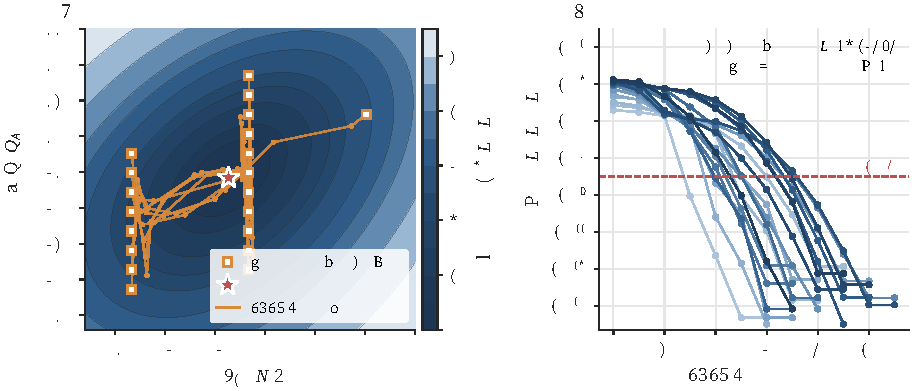
\includegraphics[width=0.88\linewidth]{images/no3/P3_F08_多起点寻优过程与收敛验证.pdf}
\caption{指数成本低预算情景的多起点寻优轨迹与局部收敛验证}
\label{fig:p3_multistart}
\end{figure}

二十个候选起点全部收敛，三条代表性路径从不同位置汇聚到表~\ref{tab:p3_anchor_allocations} 中的指数成本低预算解，相对 Loss 差距降至数值零附近。结合加密网格和完整三维复核，可排除单一初值造成的局部最优假象。全部中心解还满足成本非负、预算可行、最优值随预算不增加以及长上下文不降低 Loss 等物理门禁。

综上，模型把参数、训练 Token、质量和长上下文成本统一到预算框架，识别出“未启动提质--质量参与竞争--质量饱和后规模重新主导”的阶段变化。结论受三项边界约束：领域配比绝对强度尚未识别，质量成本为题设情景，高预算含明显外推，故只能解释为给定模型和支持域内的条件最优。

问题四接收 $3$ 种质量成本、$5$ 档上下文和 $3$ 档预算构成的 $45$ 个冻结情景，并携带最优 $(N^*,D^*,Q_A^*)$、Loss 抽样及支持标记。这些结果仅用于 Loss--Benchmark 映射，不重复作为历史能力前沿的训练样本。
